%
%  beamer_template
%
%  Created by Christopher Schommer-Pries on 2012-02-16.
%  Copyright (c) 2012. All rights reserved.
%


\documentclass{beamer}		%% The Beamer document class formats for slides. 

\usepackage{presentation}

\title{Billiards}
\author{Jonathan Allen, John Wang}
\institute[MIT]{Massachusetts Institute of Technology}
\date{November $22^\text{nd}$, 2013}

\begin{document}

\graphicspath{ {figures/} }

\frame{

\titlepage

}

\frame{
  \frametitle{Introduction}

  \begin{itemize}
    \item Billiard ball bouncing in a square
    \item Assume no gravity or friction
    \item Examine sequence of sides
  \end{itemize}
}

\subsection{Examples}

\frame{
  \frametitle{Example}

  \begin{example}
    Examine the sequence: `abab`
  \end{example}

  \begin{figure}
    \includegraphics[width=3in]{figures/abab.pdf}
  \end{figure}
}

\frame{
  \frametitle{Another Example}

  \begin{example}
    Examine the sequence: `aaabaaab`
  \end{example}

  \begin{figure}
    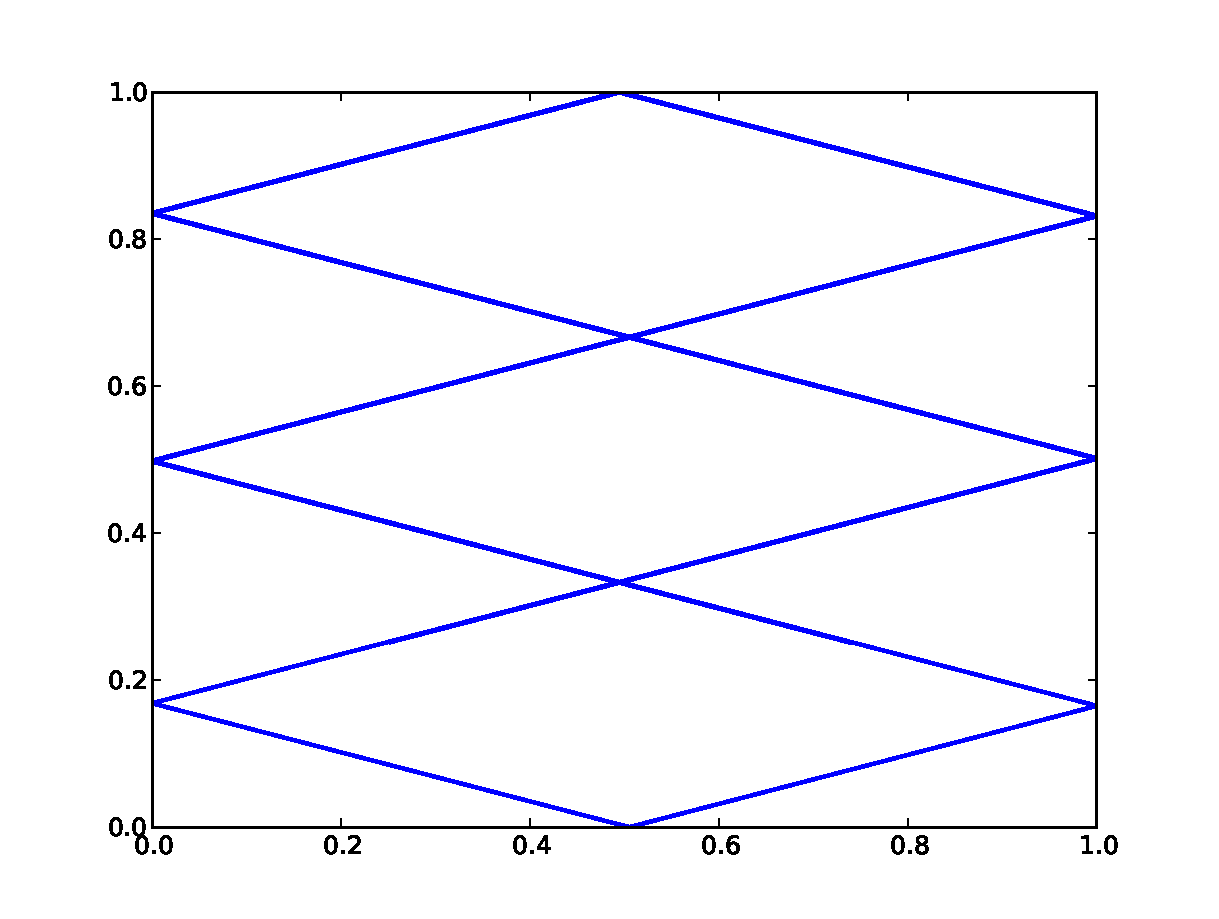
\includegraphics[width=3in]{figures/aaabaaab.pdf}
  \end{figure}
}

\subsection{Outline}

\frame{
  \frametitle{Presentation Outline}
  \tableofcontents
}

\frame{
  \frametitle{Notation}

  \begin{definition}
    A table $T$ is the unit square in $\mathrm{R}^2$. A particle $p \in T$ begins at position $\bar{x}_0 \in T$ with velocity $\bar{v}$. When the particle reaches an edge of the table, velocity is reflected about the line perpendicular to the table's edge.
  \end{definition}

  \begin{figure}
    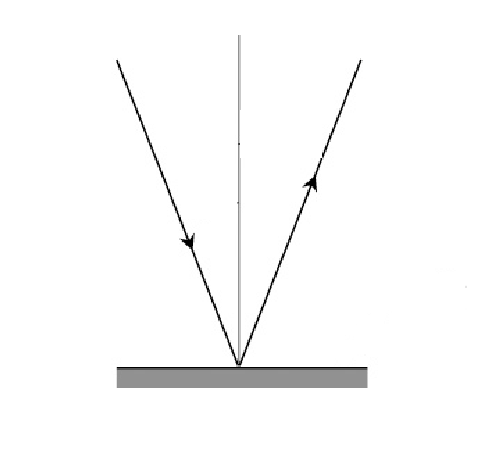
\includegraphics[width=2in]{figures/particle_collision.png}
  \end{figure}
}

\frame{
  \frametitle{Notation}
  \begin{definition}
    Sequence
  \end{definition}
}

\subsection{Problem Statement and Notation}

\frame{
  \frametitle{Problem Statement}

  Problem: What properties of s
}



\subsection{Tiling}

\frame{
  \frametitle{Representing Collision Strings}

  \begin{itemize}
    \item Reflect squares about each side to create a tiling
    \item Solutions become lines in the plane
    \item Intersections become places where collisions occur
  \end{itemize}
}

\frame{
  \frametitle{Representing Collision Strings}

  \begin{example}
    Tiling of $\vec{x}_0 = (0, 0.5)$ and $\vec{v} = (0.25, 0.25)$.
  \end{example}

  \begin{columns}
    \begin{column}{0.45\textwidth}
      \begin{figure}
        \includegraphics[width=2.1in]{abab.pdf}
      \end{figure}
    \end{column}
    \begin{column}{0.45\textwidth}
      \begin{figure}
        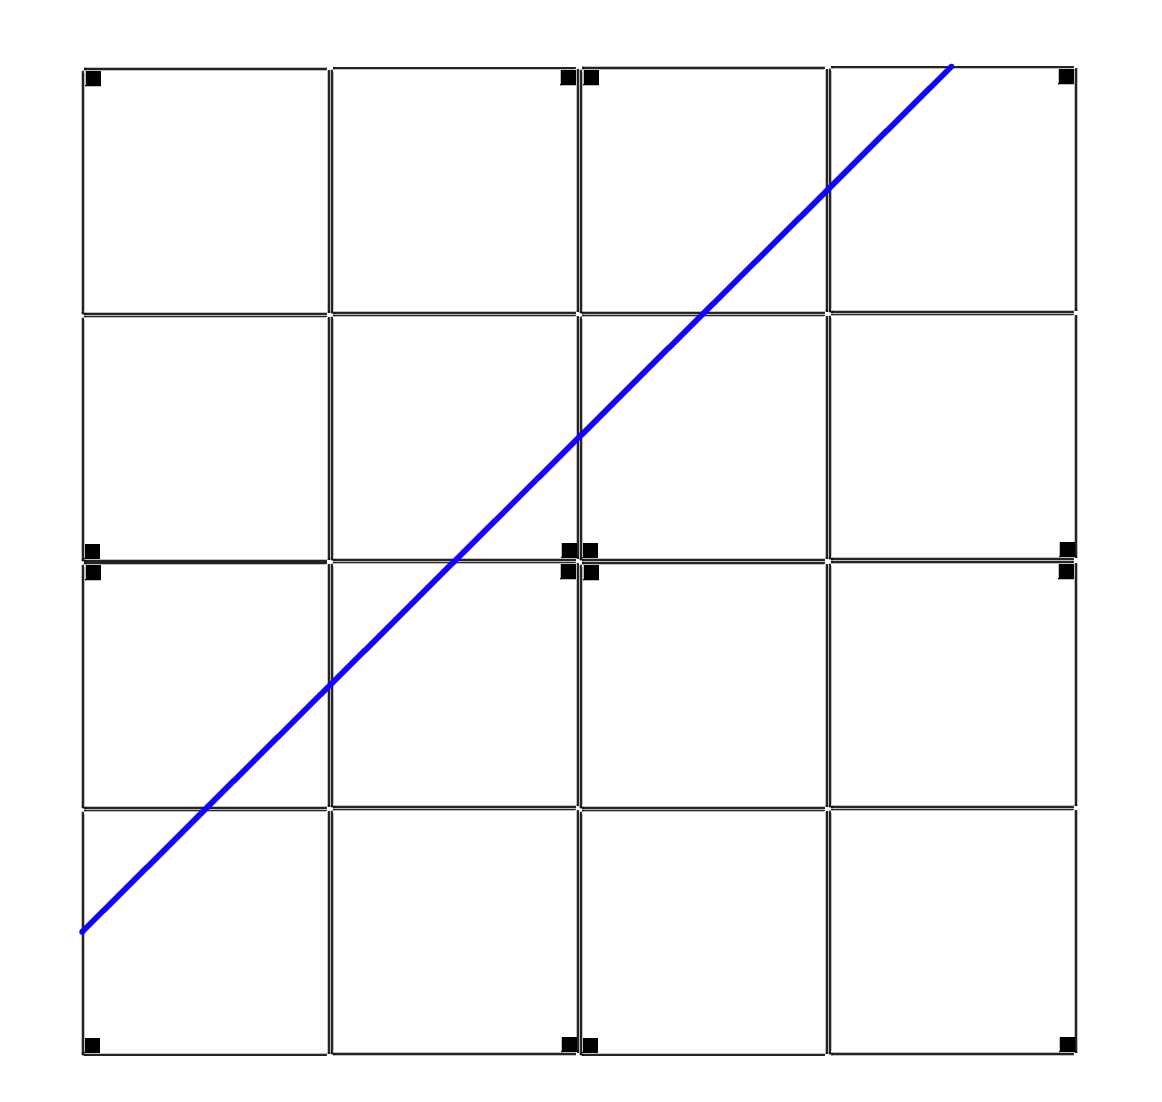
\includegraphics[width=1.7in]{tiling.png}
      \end{figure}
    \end{column}
  \end{columns}
}

\frame{
  \frametitle{Representing Collision Strings}

  \begin{example}
    Tiling of $\vec{x}_0 = (0, 0.5)$ and $\vec{v} = (0.25, 0.25)$.
  \end{example}

  \begin{columns}
    \begin{column}{0.45\textwidth}
      \begin{figure}
        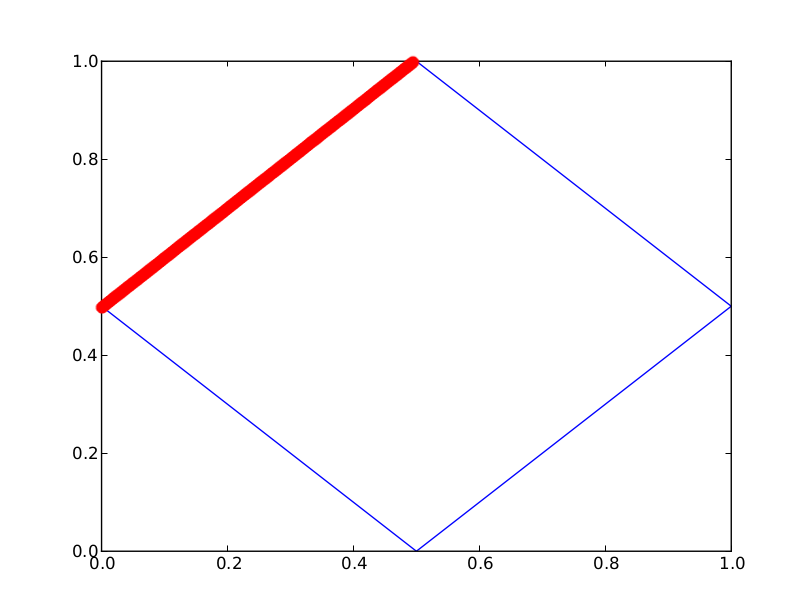
\includegraphics[width=2.1in]{tiling_real_step_1.png}
      \end{figure}
    \end{column}
    \begin{column}{0.45\textwidth}
      \begin{figure}
        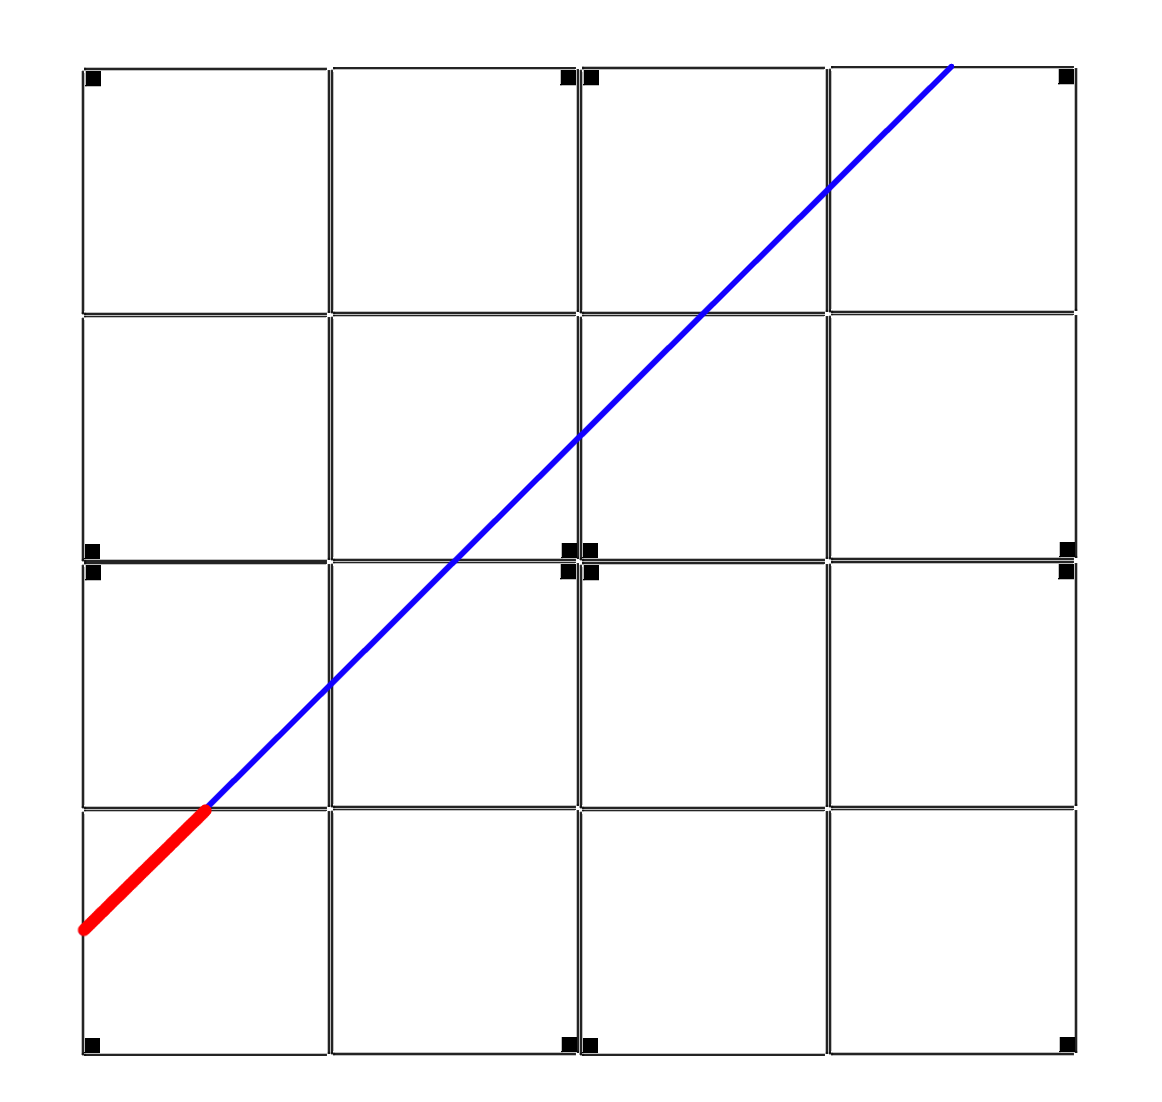
\includegraphics[width=1.7in]{tiling_tiled_step_1.png}
      \end{figure}
    \end{column}
  \end{columns}
}

\frame{
  \frametitle{Representing Collision Strings}

  \begin{example}
    Tiling of $\vec{x}_0 = (0, 0.5)$ and $\vec{v} = (0.25, 0.25)$.
  \end{example}

  \begin{columns}
    \begin{column}{0.45\textwidth}
      \begin{figure}
        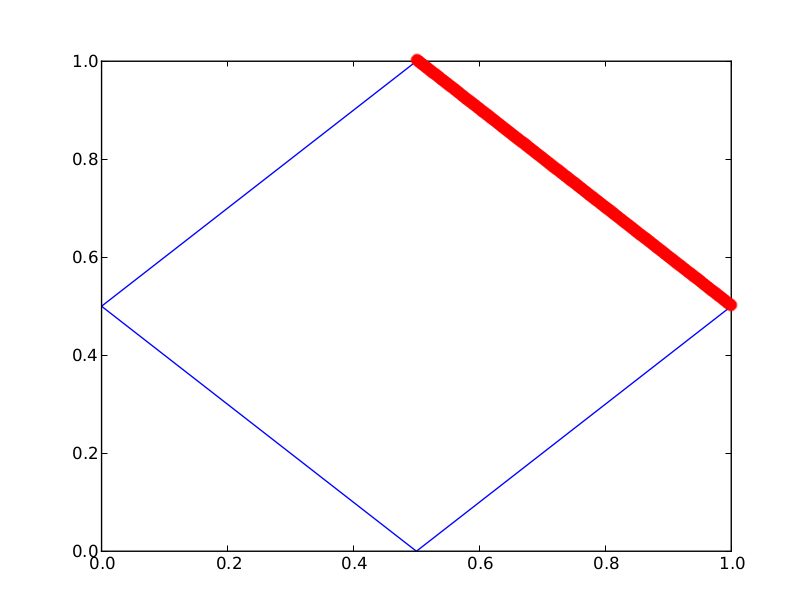
\includegraphics[width=2.1in]{tiling_real_step_2.png}
      \end{figure}
    \end{column}
    \begin{column}{0.45\textwidth}
      \begin{figure}
        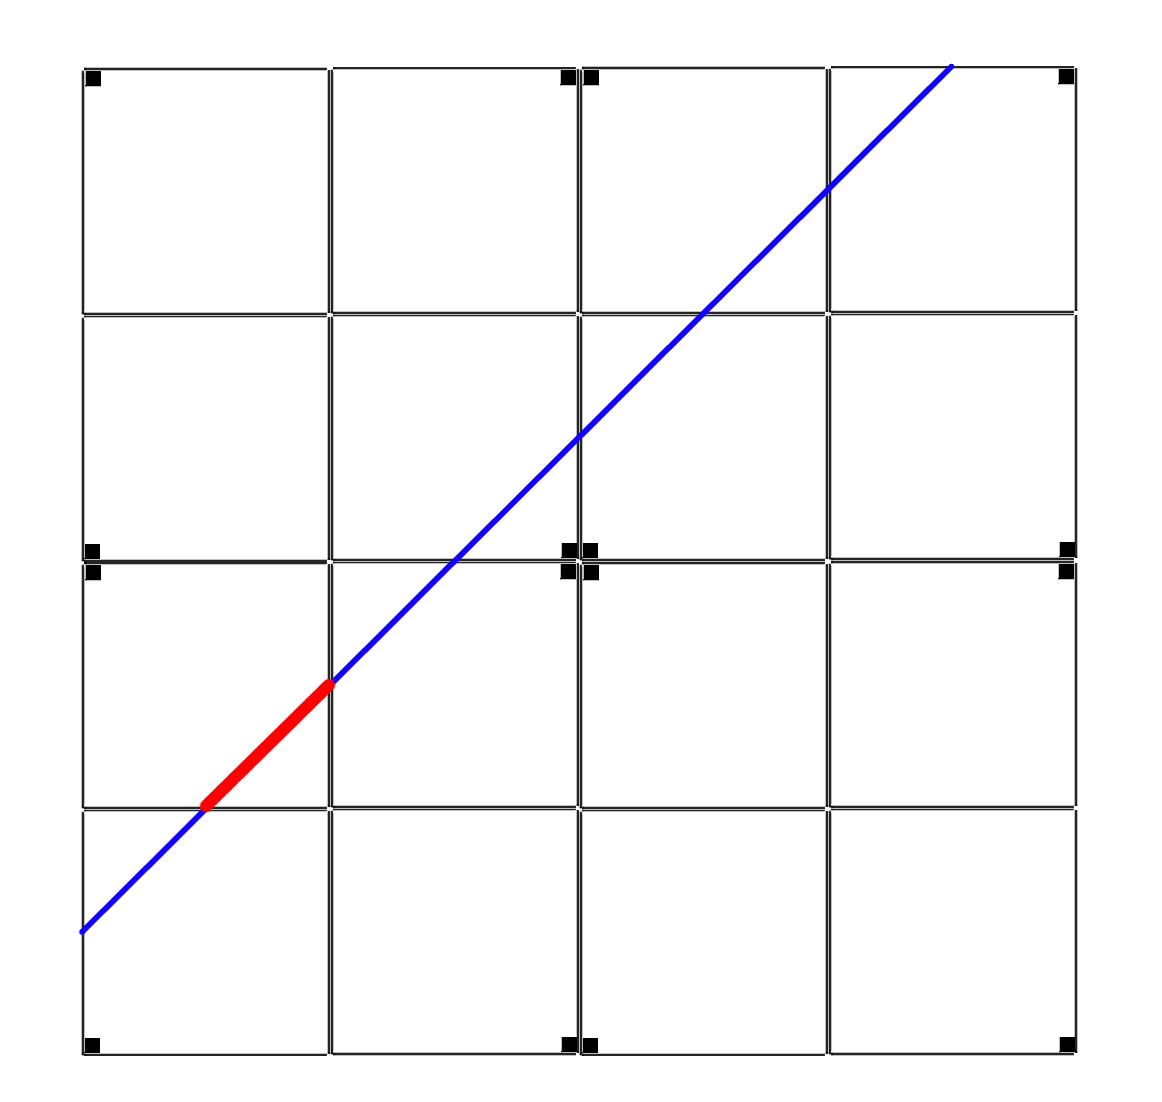
\includegraphics[width=1.7in]{tiling_tiled_step_2.png}
      \end{figure}
    \end{column}
  \end{columns}
}

\frame{
  \frametitle{Representing Collision Strings}

  \begin{example}
    Tiling of $\vec{x}_0 = (0, 0.5)$ and $\vec{v} = (0.25, 0.25)$.
  \end{example}

  \begin{columns}
    \begin{column}{0.45\textwidth}
      \begin{figure}
        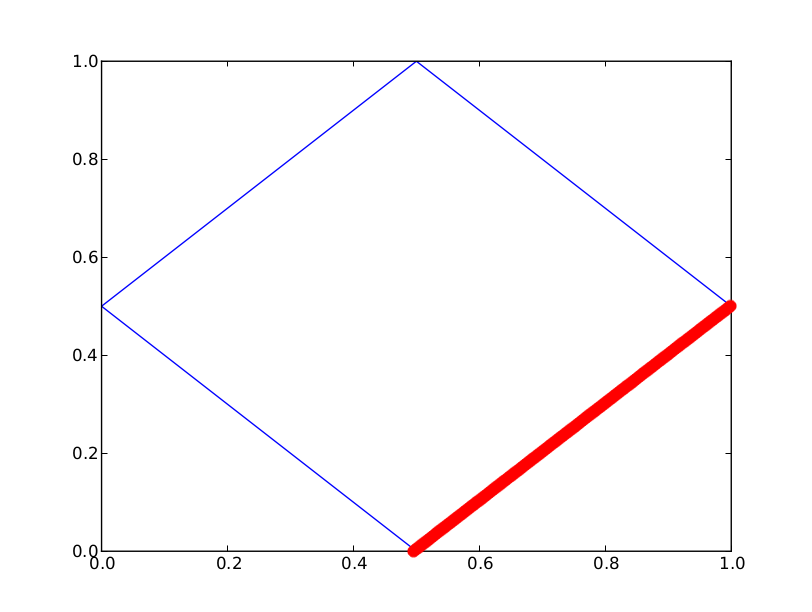
\includegraphics[width=2.1in]{tiling_real_step_3.png}
      \end{figure}
    \end{column}
    \begin{column}{0.45\textwidth}
      \begin{figure}
        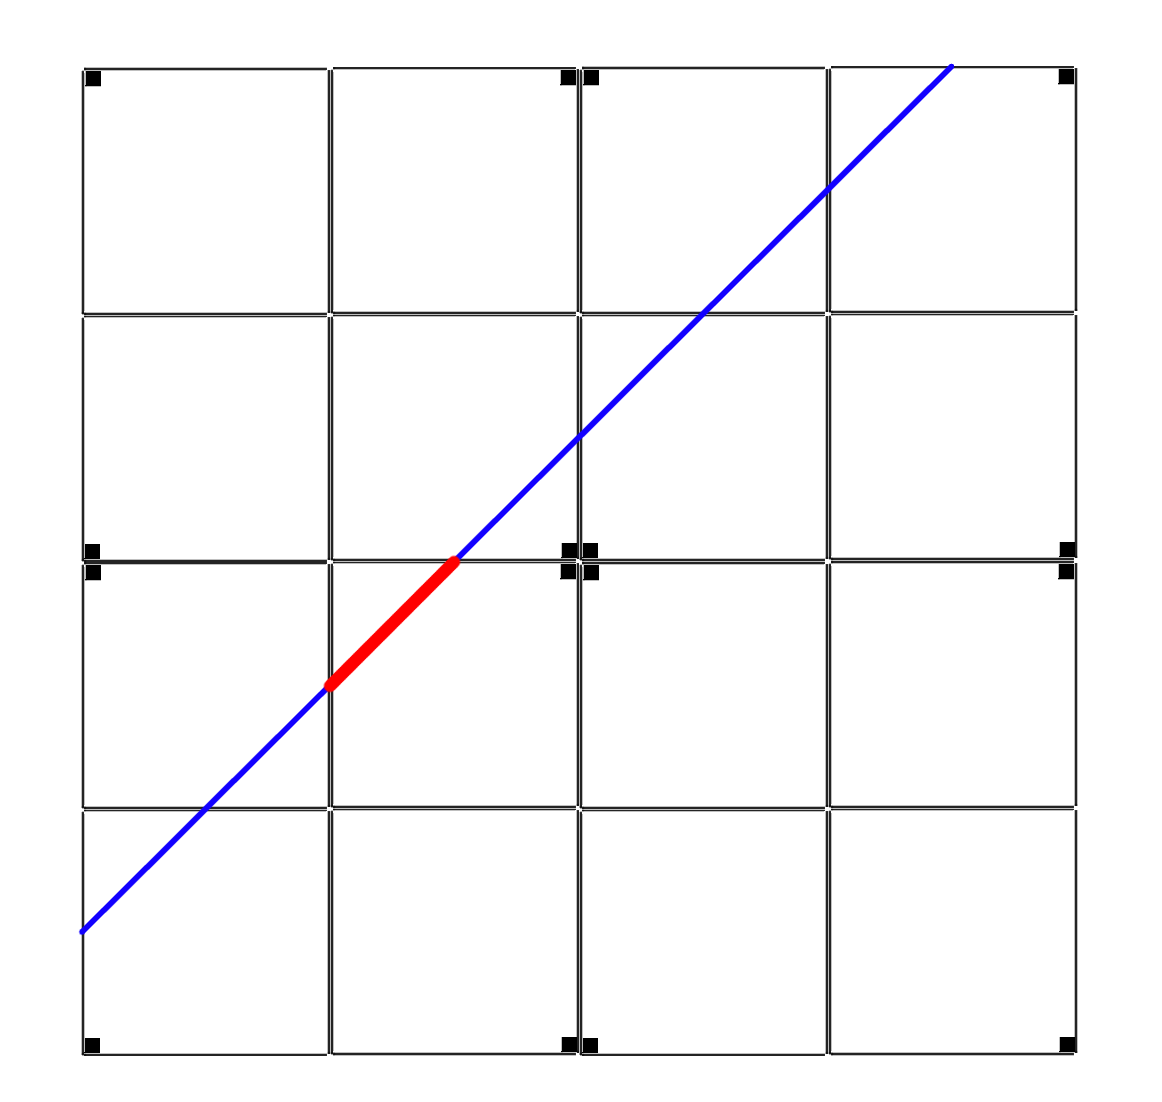
\includegraphics[width=1.7in]{tiling_tiled_step_3.png}
      \end{figure}
    \end{column}
  \end{columns}
}

\frame{
  \frametitle{Representing Collision Strings}

  \begin{example}
    Tiling of $\vec{x}_0 = (0, 0.5)$ and $\vec{v} = (0.25, 0.25)$.
  \end{example}

  \begin{columns}
    \begin{column}{0.45\textwidth}
      \begin{figure}
        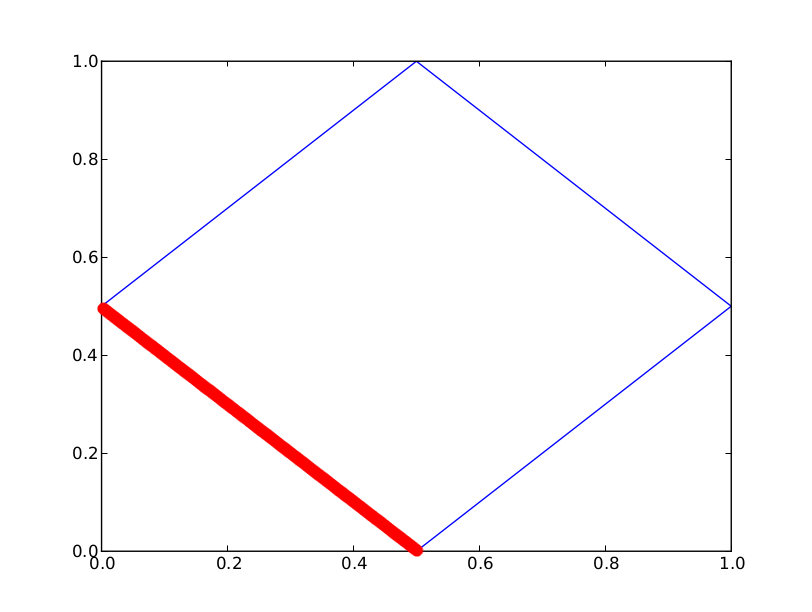
\includegraphics[width=2.1in]{tiling_real_step_4.png}
      \end{figure}
    \end{column}
    \begin{column}{0.45\textwidth}
      \begin{figure}
        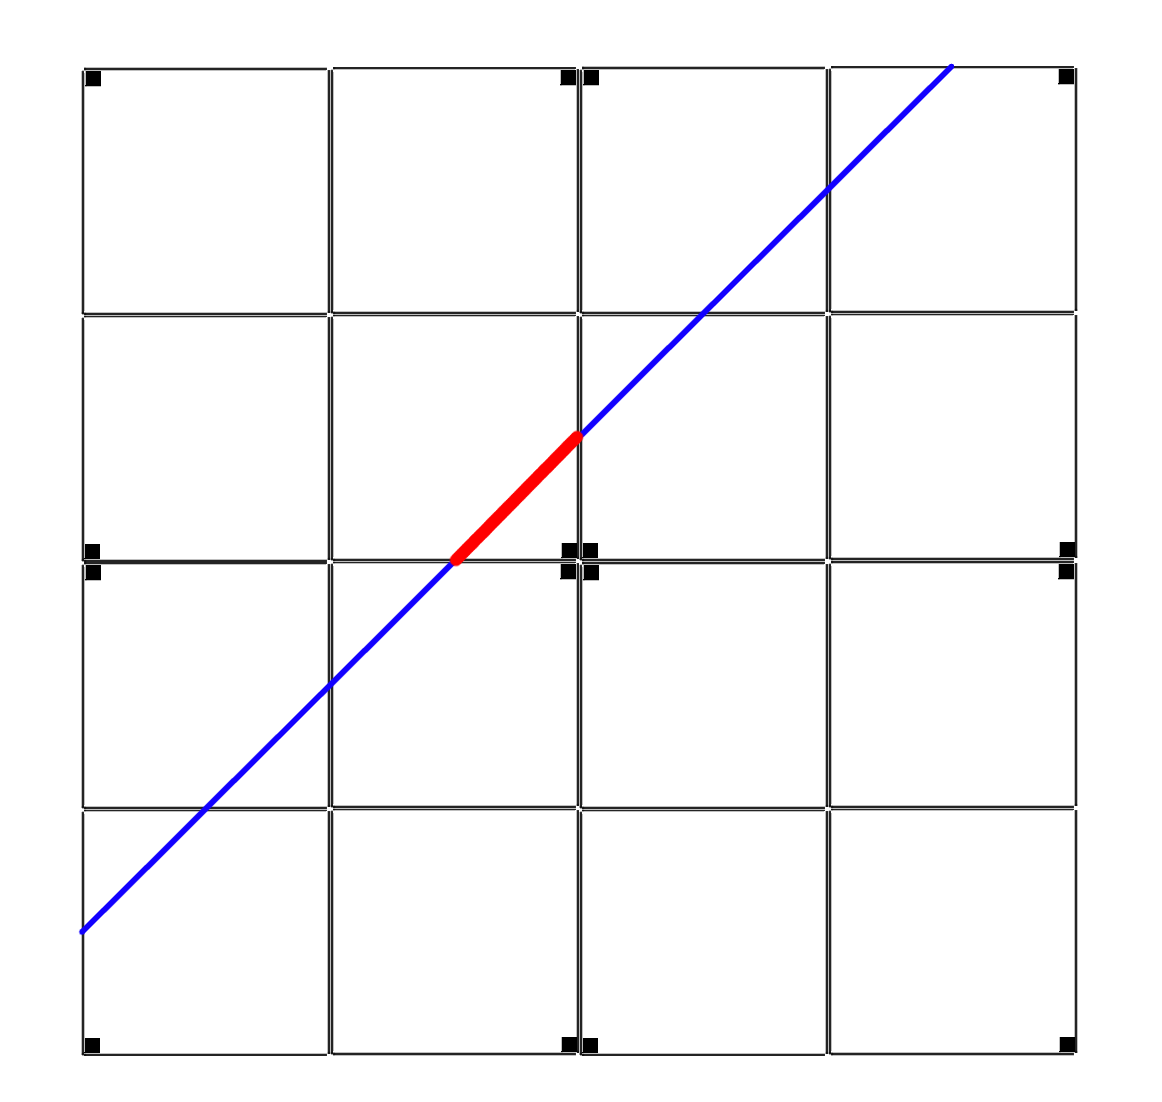
\includegraphics[width=1.7in]{tiling_tiled_step_4.png}
      \end{figure}
    \end{column}
  \end{columns}
}

\frame{
  \frametitle{Representing Collision Strings}

  \begin{example}
    Tiling of $\vec{x}_0 = (0, 0.5)$ and $\vec{v} = (0.25, 0.25)$.
  \end{example}

  \begin{columns}
    \begin{column}{0.45\textwidth}
      \begin{figure}
        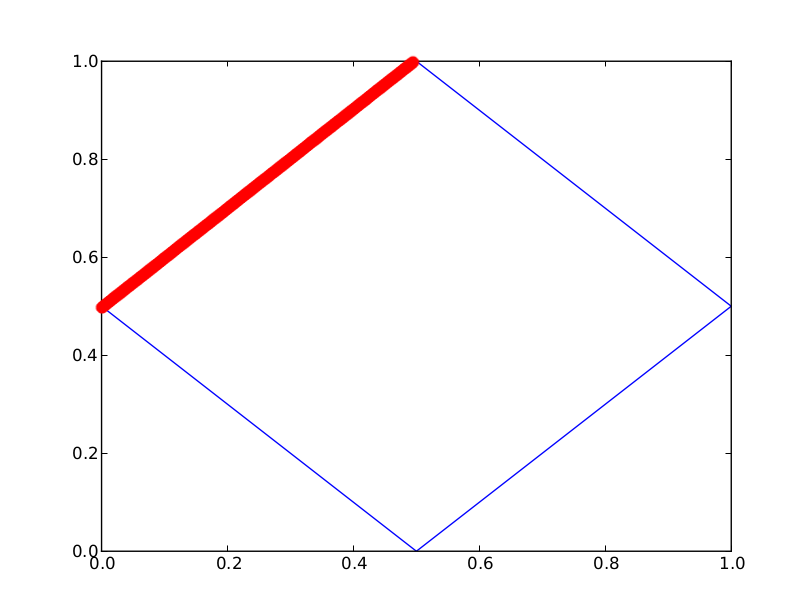
\includegraphics[width=2.1in]{tiling_real_step_1.png}
      \end{figure}
    \end{column}
    \begin{column}{0.45\textwidth}
      \begin{figure}
        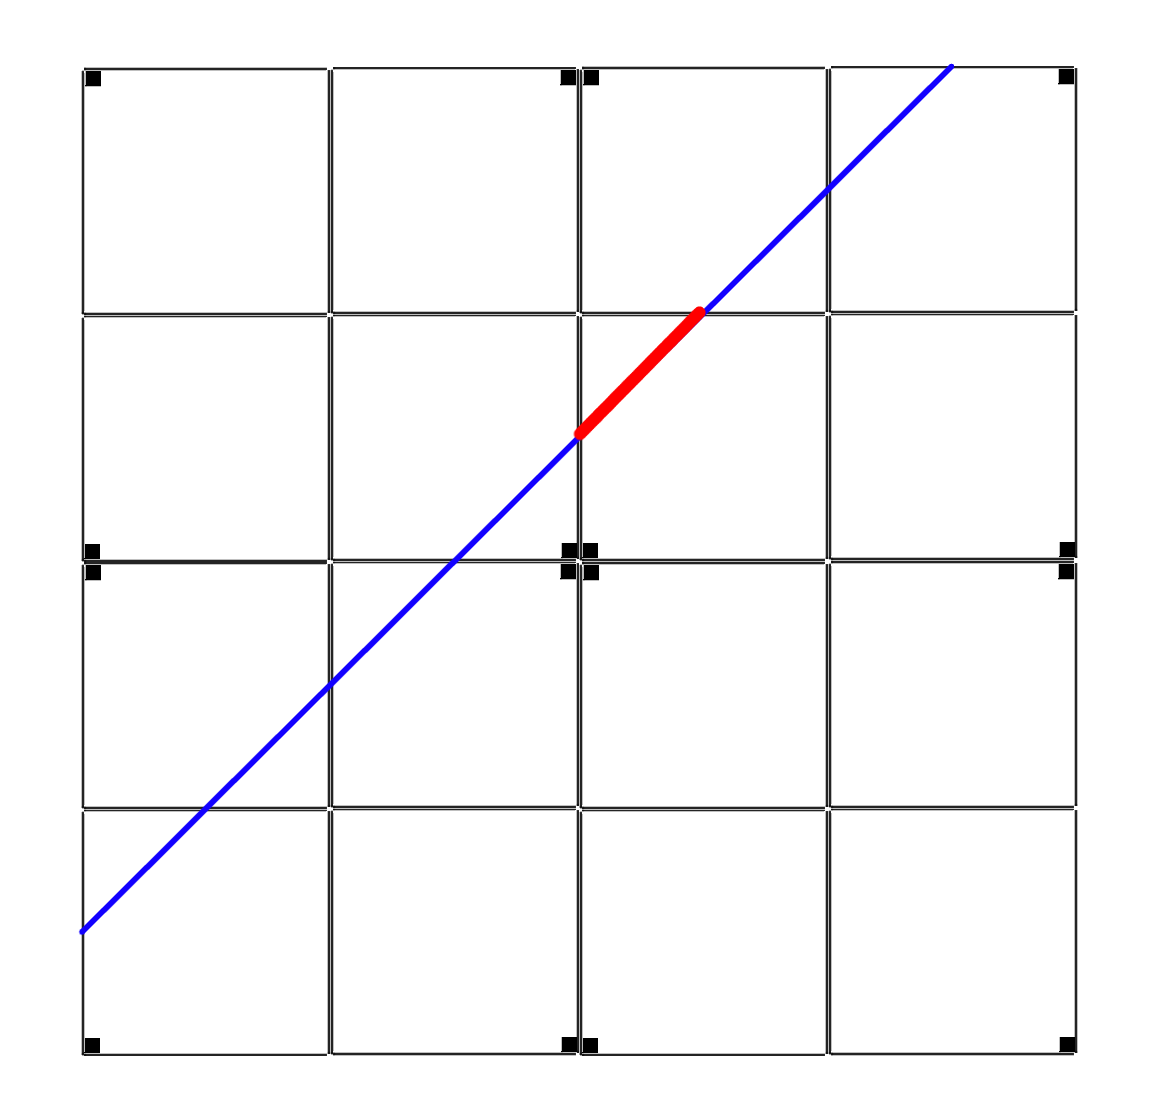
\includegraphics[width=1.7in]{tiling_tiled_step_5.png}
      \end{figure}
    \end{column}
  \end{columns}
}

\frame{
  \frametitle{Representing Collision Strings}

  \begin{example}
    Tiling of $\vec{x}_0 = (0, 0.5)$ and $\vec{v} = (0.25, 0.25)$.
  \end{example}

  \begin{columns}
    \begin{column}{0.45\textwidth}
      \begin{figure}
        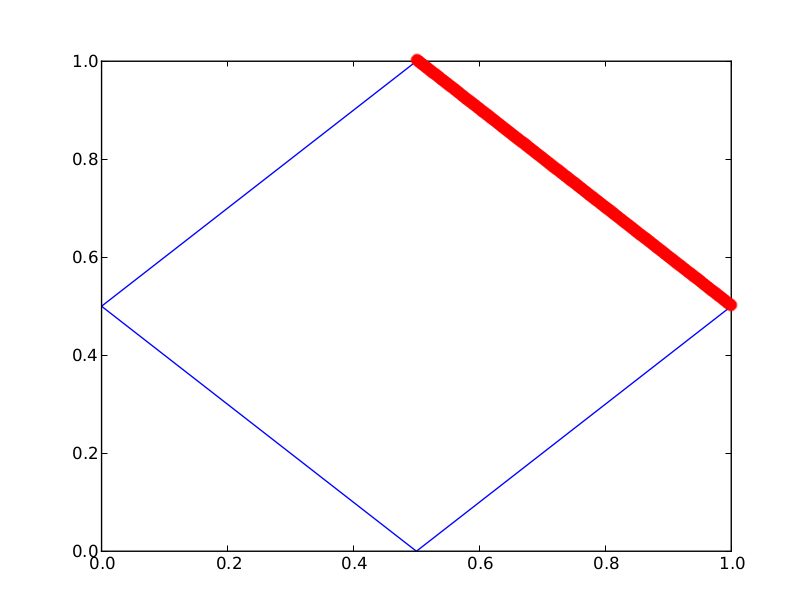
\includegraphics[width=2.1in]{tiling_real_step_2.png}
      \end{figure}
    \end{column}
    \begin{column}{0.45\textwidth}
      \begin{figure}
        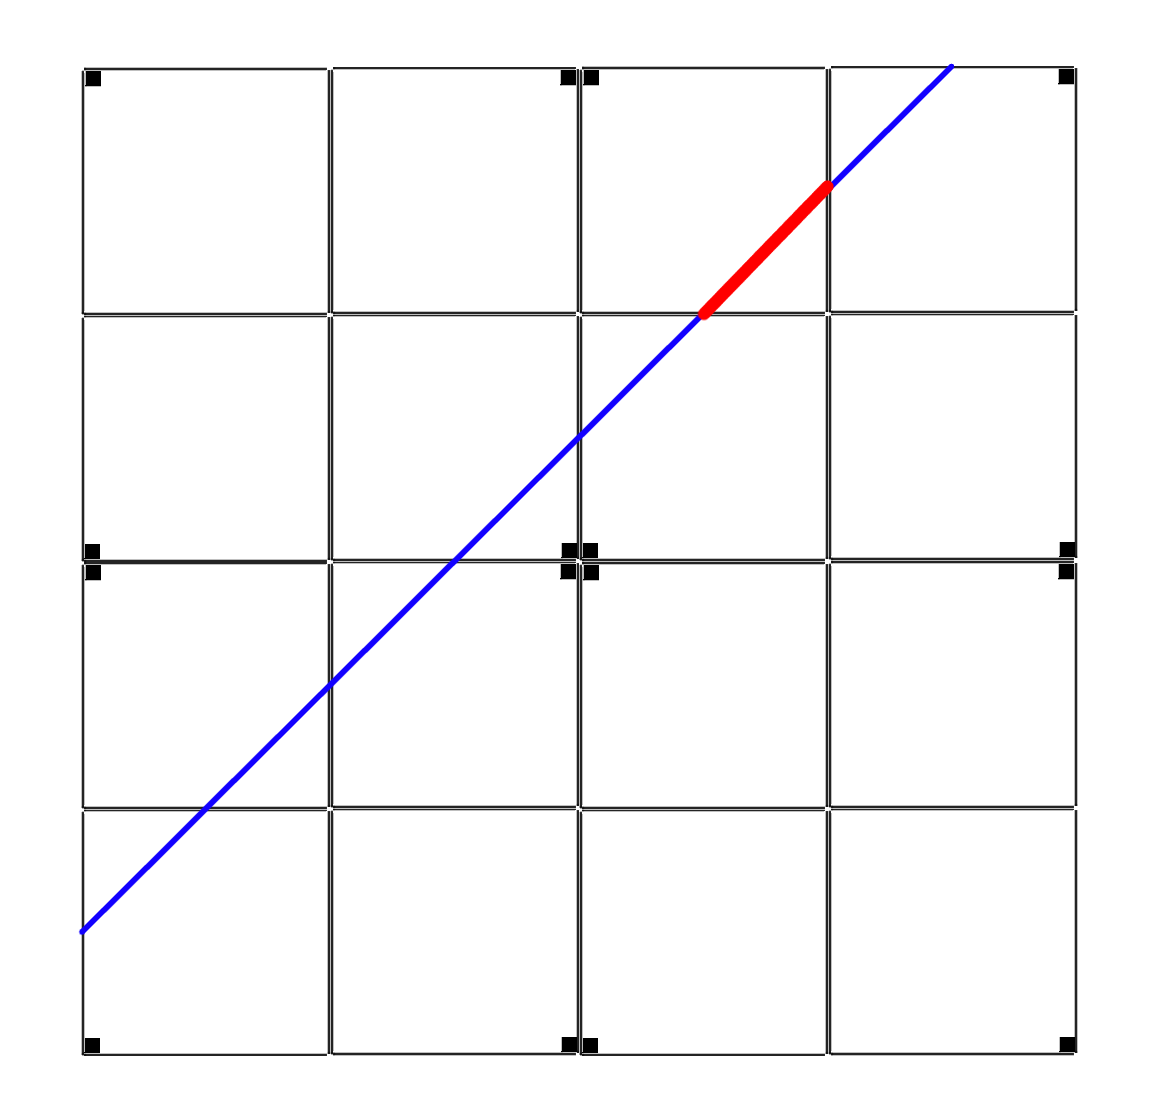
\includegraphics[width=1.7in]{tiling_tiled_step_6.png}
      \end{figure}
    \end{column}
  \end{columns}
}

\frame{
  \frametitle{Representing Collision Strings}

  \begin{example}
    Tiling of $\vec{x}_0 = (0, 0.5)$ and $\vec{v} = (0.25, 0.25)$.
  \end{example}

  \begin{columns}
    \begin{column}{0.45\textwidth}
      \begin{figure}
        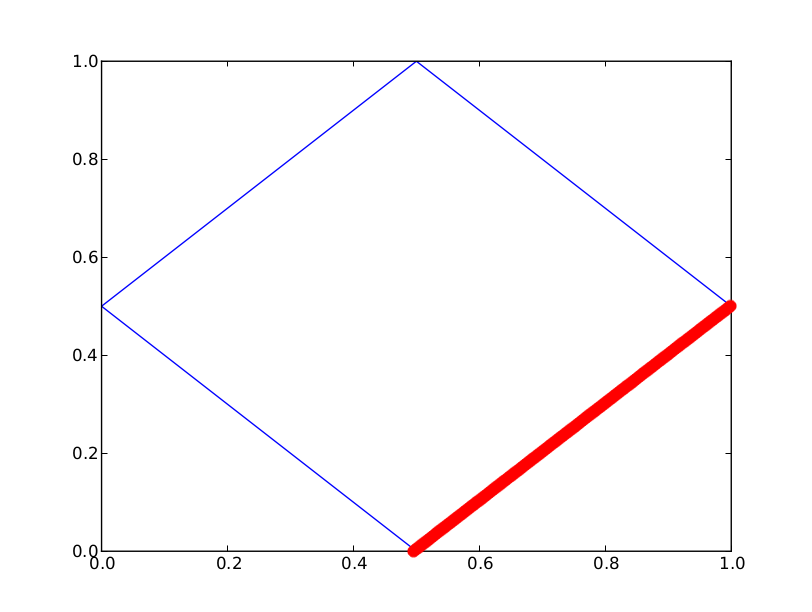
\includegraphics[width=2.1in]{tiling_real_step_3.png}
      \end{figure}
    \end{column}
    \begin{column}{0.45\textwidth}
      \begin{figure}
        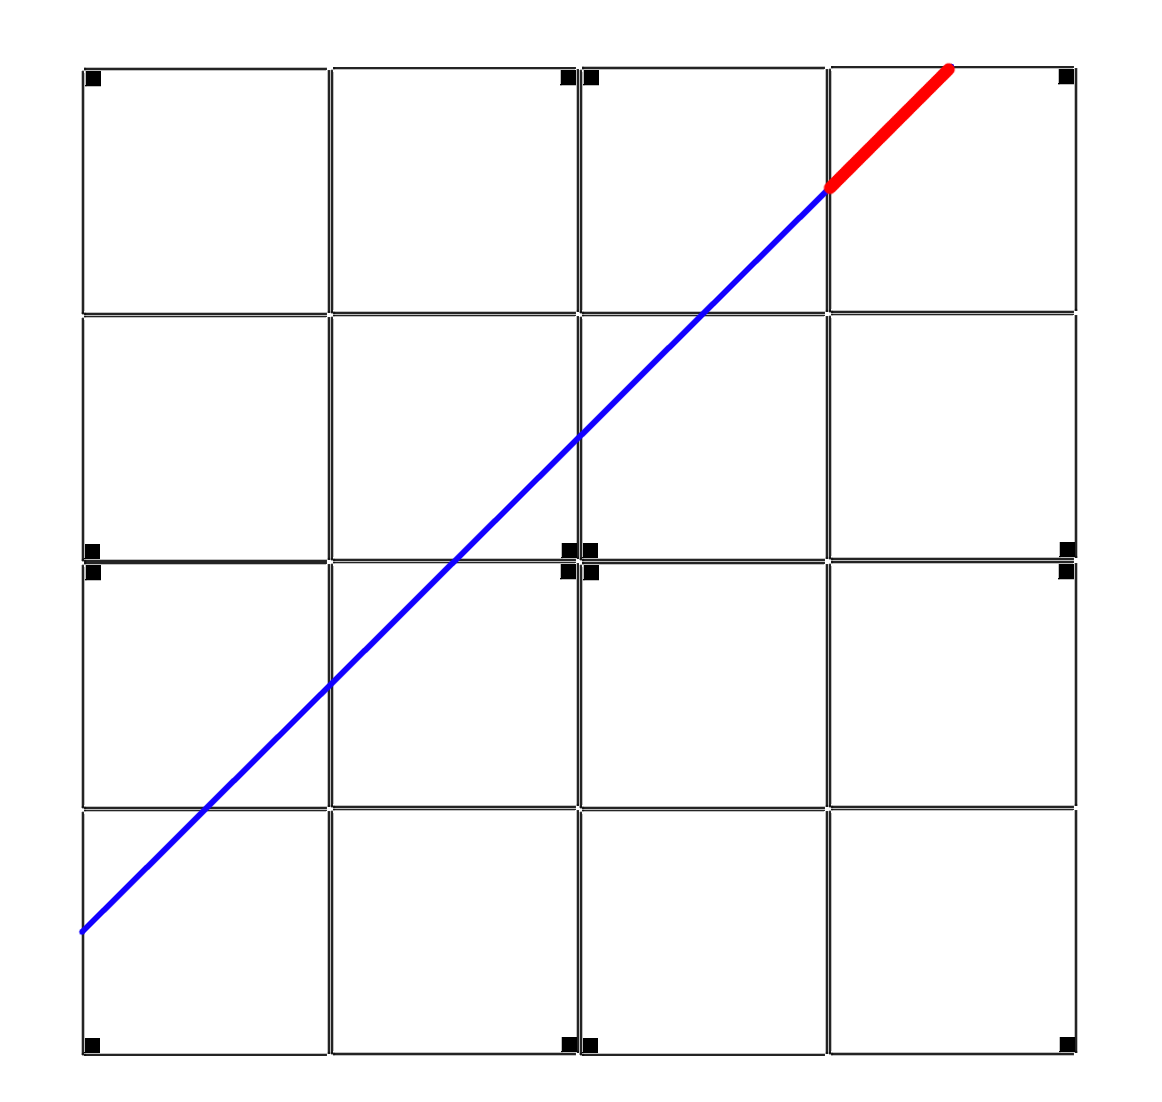
\includegraphics[width=1.7in]{tiling_tiled_step_7.png}
      \end{figure}
    \end{column}
  \end{columns}
}

\subsection{1-dimensional Problem}

\frame{
  \frametitle{Sequence Characterization}

  \begin{multline*}
    \begin{array}{cccccccccc}
      \underbrace{aaa} & b & \underbrace{aa} & b & \underbrace{aa} & b & \underbrace{aaa} & b & \underbrace{aa} & b \\
      3 && 2 && 2 && 3 && 2 &
    \end{array}\\
    \begin{array}{cccccccc}
      \underbrace{aa} & b & \underbrace{aaa} & b & \underbrace{aa} & b & \underbrace{aaa} & \dots \\
      2 && 3 && 2 && 3 & \dots
    \end{array}
  \end{multline*}
}

\frame{
  \frametitle{Sequence Characterization}

  \begin{gather*}
    \begin{array}{cccccccc}
      3 & \underbrace{22} & 3 & \underbrace{22} & 3 & \underbrace{2} & 3 & \dots\\ 
      & 2 && 2 && 1 & \dots
    \end{array}
  \end{gather*}
}


\frame{

\frametitle{Trajectory Calculation Algorithm}
	
\begin{enumerate}
\item Let $i = 0$
\item 
\end{enumerate}

}

\subsection{Cubes}

\frame{
  \frametitle{Extensions to Cubes}

  \begin{itemize}
    \item Assign $x$, $y$, and $z$ as the opposite pairs of faces of a cube.
    \item Characterize sequences of $x$, $y$, and $z$ collisions.
  \end{itemize}
}

\frame{
  \frametitle{Intuition}

  \begin{itemize}
    \item Examine collisions in $xy$, $yz$, and $xz$ planes.
    \item Movement in each plane is independent.
    \item Combine $xy$, $yz$, and $xz$ collision sequences to get final sequence.
  \end{itemize}
}

\frame{
  \frametitle{Example}

  \begin{example}
    $xy$ sequence: $xxyyxx$
    $yz$ sequence: $zzyzyz$
    $xz$ sequence: $xxzzzx$
  \end{example}
}




\frame{
This is a slide!
}


\frame{
\frametitle{This slide has a title!}

\pause
Wow!
\pause

You can also make lists...
\begin{itemize}
	\item with an item \pause
	\item and another item.
\end{itemize}

}


\frame{
You can typeset equations just as in latex:
\[
\int_0^1 x\, dx = 1/2,
\]
or
$$
\sum_{i = 1}^\infty i = -\frac{1}{12}
$$
or
\begin{equation*}
1 - 1 + 1 - \cdots = \frac{1}{2}.
\end{equation*}

}


\frame{
If you want a number for an equation, do it like this:
\begin{equation}\label{eq:first-equation}
\lim_{n \to \infty}\, \sum_{k = 1}^n \frac{1}{k^2} = \frac{\pi}{6}.
\end{equation} %
This can then be referred to as \eqref{eq:first-equation}, which is much easier than
keeping track of numbers by hand. To group several equations, aligning on the $=$ sign, do
it like this:
\begin{align*}
x_1 + 2x_2 + 3x_3 &= 7 \\ y &= mx + c \\ &= 4x - 9.
\end{align*}
}

\frame{
\begin{theorem}[my great theorem]
	This theorem proves everything.
\end{theorem}

\begin{example}
	For example it proves \alert{this}! % "alert" makes it red
\end{example}

}



\end{document}

